\part{Navigation meshes}
\frame{\partpage}

\begin{frame}{Pathfinding in videogames}
	\begin{itemize}
		\pause\item A$^*$ works on any \textbf{graph}
		\pause\item But what if the game world is not a graph? E.g.\ complex 3D environments
	\end{itemize}
\end{frame}

\begin{frame}{Waypoint navigation}
	\begin{columns}
		\begin{column}{0.4\textwidth}
			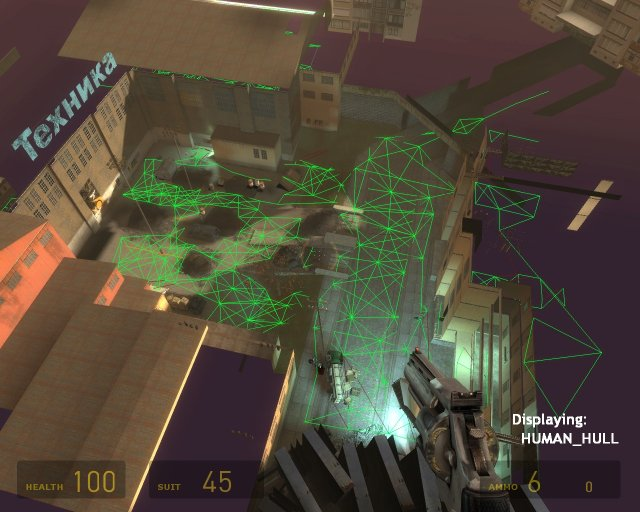
\includegraphics[width=\textwidth]{nodegraph} % https://developer.valvesoftware.com/wiki/Nodegraph
		\end{column}
		\begin{column}{0.58\textwidth}
			\begin{itemize}
				\pause\item Manually place graph nodes in the world
				\pause\item Place them at key points, e.g.\ in doorways, around obstacles
				\pause\item Works, but...
					\begin{itemize}
						\pause\item More work for level designers
						\pause\item Requires lots of testing and tweaking to get natural-looking results
						\pause\item No good for dynamic environments
					\end{itemize}
			\end{itemize}
		\end{column}
	\end{columns}
\end{frame}

\begin{frame}{Navigation meshes}
	\begin{columns}
		\begin{column}{0.4\textwidth}
			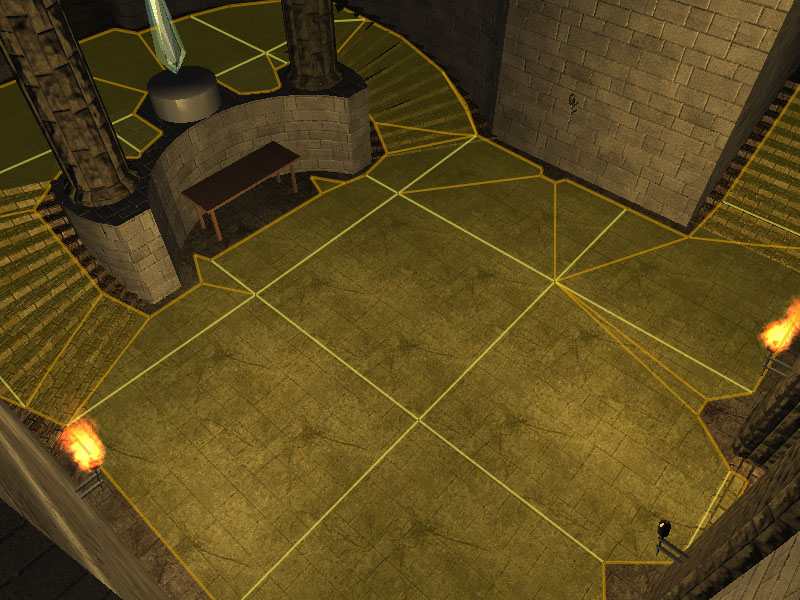
\includegraphics[width=\textwidth]{navmesh} % http://www.crystalspace3d.org/blog/leonardord?cat=53
		\end{column}
		\begin{column}{0.58\textwidth}
			\begin{itemize}
				\pause\item Automatically generate navigation graph from level geometry
				\pause\item Basic idea:
					\begin{itemize}
						\pause\item Filter level geometry to those polygons which are \textbf{passable}
							(i.e.\ floors, not walls/ceilings/obstacles)
						\pause\item Generate graph from polygons
					\end{itemize}
			\end{itemize}
		\end{column}
	\end{columns}
\end{frame}

\begin{frame}{Meshes to graphs}
	\begin{center}
		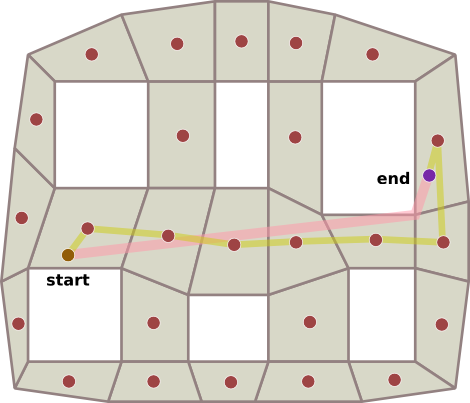
\includegraphics[width=0.6\textwidth]{polygon-navmesh-faces}
		% http://theory.stanford.edu/~amitp/GameProgramming/MapRepresentations.html
		
		Centres of polygons
	\end{center}
\end{frame}

\begin{frame}{Meshes to graphs}
	\begin{center}
		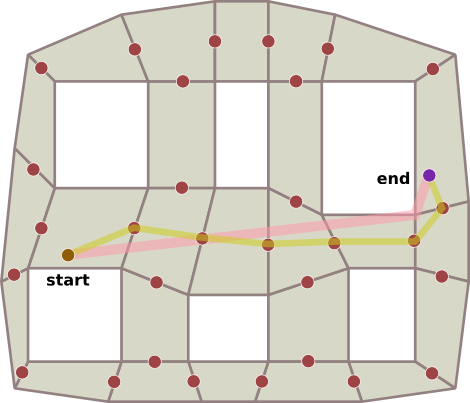
\includegraphics[width=0.6\textwidth]{polygon-navmesh-edges}
		% http://theory.stanford.edu/~amitp/GameProgramming/MapRepresentations.html
		
		Centres of edges
	\end{center}
\end{frame}

\begin{frame}{Meshes to graphs}
	\begin{center}
		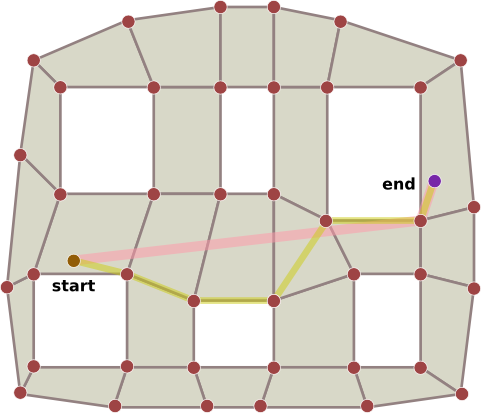
\includegraphics[width=0.6\textwidth]{polygon-navmesh-vertices}
		% http://theory.stanford.edu/~amitp/GameProgramming/MapRepresentations.html
		
		Vertices of polygons
	\end{center}
\end{frame}

\begin{frame}{Meshes to graphs}
	\begin{center}
		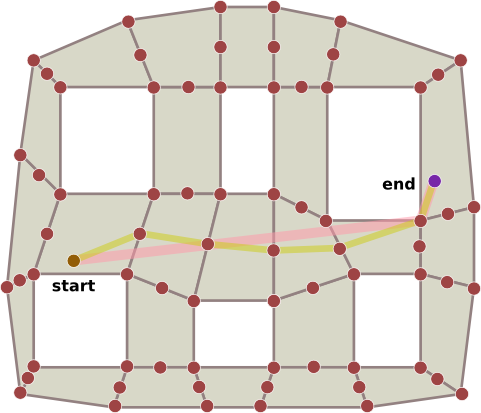
\includegraphics[width=0.6\textwidth]{polygon-navmesh-edges-and-vertices}
		% http://theory.stanford.edu/~amitp/GameProgramming/MapRepresentations.html
		
		Hybrid approach: edges and vertices
	\end{center}
\end{frame}

\begin{frame}{Following the path}
	\begin{itemize}
		\pause\item \textbf{Funnelling}: like string pulling but for navigation meshes
			\begin{itemize}
				\pause\item \url{http://digestingduck.blogspot.co.uk/2010/03/simple-stupid-funnel-algorithm.html}
				\item \url{http://jceipek.com/Olin-Coding-Tutorials/pathing.html}
			\end{itemize}
		\pause\item \textbf{Steering}: don't have your AI agent follow the path exactly, but
			instead try to stay close to it
		\pause\item \textbf{Dynamic environments}: may need to re-run pathfinder if environment changes
			(e.g.\ movable obstacles, destructible terrain)
	\end{itemize}
\end{frame}

